\documentclass[10pt,letterpaper]{article}

\usepackage{geometry}
\usepackage{hyperref}
\usepackage{graphicx}
\usepackage{listings}

\geometry{body={7.0in, 10.0in},left=0.75in,top=0.75in}

\hypersetup{colorlinks = true,urlcolor = black,pdfauthor = {Alexander Brown},pdfkeywords = {},pdftitle = {CS22310 - Assignment 1: Website usability mini-project},pdfsubject = {CS22310 - Assignment 1},pdfpagemode = Default}

\setlength\parindent{0em}
\setlength{\parskip}{1ex plus 0.5ex minus 0.2ex}
%\setcounter{tocdepth}{2}1

\title{CS22310 - Assignment 1: Website usability mini-project}
\author{Alexander Brown}
\begin{document}
  \maketitle
%  \tableofcontents
  \section{Applying web design guidelines to three sites}
      The specific purpose I shall be approaching each of the following website with is to purchase and/or download a version of the operating system for a new, but typical mid-range laptop.
    
    \subsection{Microsoft}
      \url{http://www.microsoft.com}
      
      From the homepage I straight away noticed the menu, of which the second option was for Windows. Upon hilighting a drop down menu appeared, however not entirely sure which option to chose I decided just to click on the menu link, assuming it would just take me to the Windows page. However this action only cause the drop down menu to close and I had to move off the item then back onto it again to get it back (I discovered later that one could click on the item again to bring the menu back).
      
      This time I selected the "All Windows Products" option, on this page I was greeted by a new page (with a slightly different format) an ordered list of the Windows operating systems, the newest (Windows 7) at the top, above the page fold. Most of the rest were below the fold.
      
      After quickly reading the blurb for Windows 7, I decided that this version was probably the best and, by clicking on the Windows 7 logo, continued to the Windows 7 homepage.
      
      Skipping past the flash banner, sure that I wouldn't need any of the navigation as I was already on the page I wanted to be on, I was disappointed not to find a simple "Get it now" button. It was only after I reached the page fold that I looked above the flash banner, to find a very small menu link to "Get Windows 7".
      
      The next page gave me two options; one for considering Windows 7 on a new PC, and one for Windows 7 on a current PC. My (imaginary) laptop being new, I chose the first option. This however took me to a page devoted to buying computers and not Windows 7.
      
      Going back using the browser, I chose the other option. Again a large flash box with unnecessary products took up the majority of the screen and I was forced to scroll below the page fold to chose the "Buy it now" option for Windows 7 (note that it was the top left product).
      
      From this I got the product information page, again I had to select "Buy now", which took me to another page, again differently formatted. From this I could then have proceded to the checkout and had the operating system delivered.
      
      \subsubsection{Conclusions}
	The design was generally quite good, however a lot of advertisment for other products meant that a fair amount of information was hidden below the page fold.
	Because Microsoft is such a big company a universal style cannot really be expected, however it was notable the difference in style between the sections. The Microsoft main pages (homepage and cart) were actually nicer to look at than the Windows pages.
	
	The navigation often got confusing, the menu items on the homepage really should have been clickable and, as mentioned earlier, the advertisement ocasionally obscured important menu options. The Windows submenus were just textual links and not really obvious that they were menu options.
	
	It wasn't always obvious where I was on the website either (i.e. no breadcrumbs) but the worst offender was being taken to the shop despite just wanting to buy Windows 7 straight off it's page.
	
	
      
    \subsection{Ubuntu}
      \url{http://www.ubuntu.com}
      
      Looking first at the menu, I found options for "Desktop" and "Notebook", but no options for Laptops. Looking further down the page I found a very simple option for "Download Ubuntu".
      
      From this page I had options to download the ISO file and a few options (set by default to the latest and reccommended versions). Finally there was a large button to start the download.
      
      Further down this page there was also information on how to create a CD and install the system.
      
      \subsubsection{Conclusions}
	The design was very crisp and clear, although to be very critical there could have been a little more padding between the menu items. Also I found some of the options were right-aligned, when it would have been more natural to have them on the left.
	
	The navigation was a little unclear due to there being no laptop option. However this aside, all the common options were obviously available. There wasn't much in the way of local navigation but, as all the options were generally at the top of the page, this mattered little.
	
	Interestingly, looking through the rest of the website, the colour scheme changed for server options and I found the text on these pages difficult to read.
    
    \subsection{Oracle}
      \url{http://www.oracle.com}
      
      The first port of call on the Oracle site was the "Products and Services" menu item which brought up a sub menu. After a little while looking through the small text, I found an option for Solaris 11.
      
      This took me to what seemed like an overview page, however it took a while looking through all the local submenus to just find the download menu. Clicking on the "Download Oracle Solaris 11" option here took me to the downloads page.
      
      Here I automatically clicked on the "Download for x86 - Text install" (being the first option I thought would work with my laptop). This gave me a pop-up error saying I had to accept the license agreement before downloading.
      
      I found the check box above the link, selected accept (after reading through the terms) and was taken to a login screen. From here I entered my details and was given the ISO file to download.
      
      \subsubsection{Conclusions}
	The design was very busy, a lot of small text with a lot of detail in many sections. It wasn't always obvious what was a link and what was just text.
	
	The navigation was appalling, however I find this a little unfair to use this against Oracle as their main service is databases. There was a much easier way to download Solaris via \url{http://www.oracle.com/Sun/Solaris_OS}.
	Yet Ubuntu and Windows managed to do the same with less confusion. I feel a regular use probably would have given up long before they could have found the download option.
	
	There was, however, the use of breadcrumbs to show exactly where the user was.

\newpage
 
  \section{Design and evaluation of your own website}
	\url{http://hci.alexanderdbrown.com}
	
	\begin{figure}[htb]
		\begin{center}
		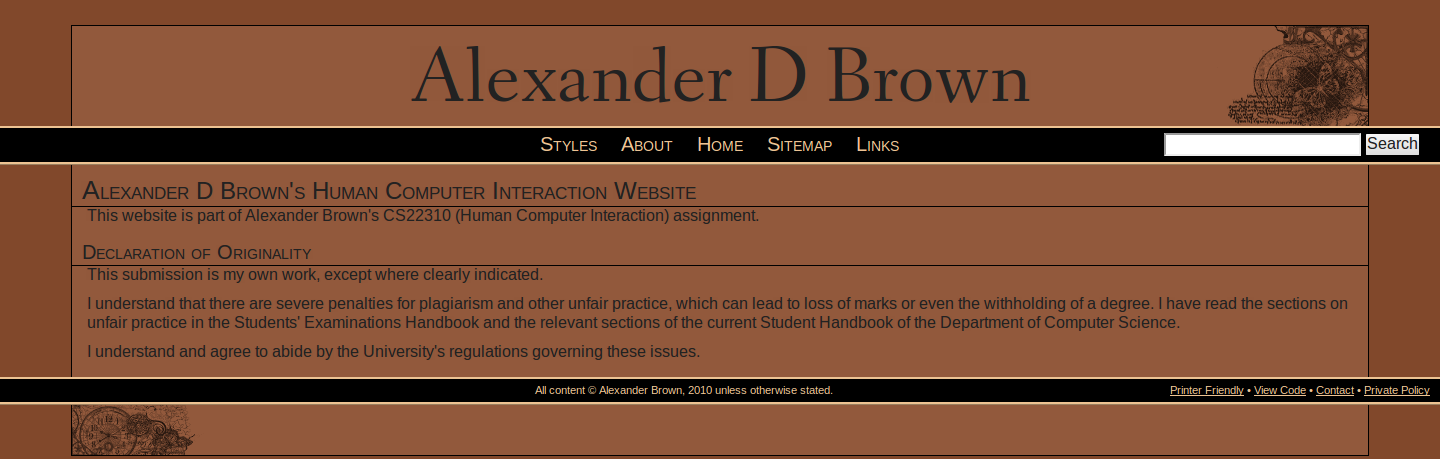
\includegraphics[scale=0.3]{overview.png}
		\caption{Overview of the Website}
		\end{center}
	\end{figure}

	This site is designed to be a personal website with a somewhat steampunk look to it.

	The first design choice I made was to have a menu bar across the top of the page; due to the nature of the website there would be very little need for sub-menus (for which I find menus on the left side of the page are more suited to). Following Krug's first law of design usability ``Don't make me think''\cite{krug06} I made this menu bar as obvious as possible, inverting the colours from the rest of the page. I also added in a search box to allow for quick access to content not made obvious by the items in the menu, this I left as the default style for a search box, to ensure it registered to the user as a search box.

	When adding content to the Menu Bar I remembered Miller's Law\cite{miller56} (on average the human mind can only store 7$\pm$2 items in Working Memory, not going into any depth on chunking, time, distraction, etc.) and took the approach of having only 5 items in the menu so that they could easily be recalled by the vast majority of users. 

	To distinguish titles from the rest of the page I used small captials and a horizontal rule, allowing the page to be broken into easily distinguishable sections, should the content be sufficiently long enough. The content itself is slightly indented from the headers for a similar reason. I also kept a very standard link style for links not in the menu (underlined with a slightly different colour from the rest of the text) so they could easily be picked out from the text. I decided against using breadcrumbs to keep the page style simple, as the website is not large enough to warrent including them.

	With the paragraphs I decided to go with a small gap inbetween paragraphs rather than an indent (which I find doesn't suit websites) to distinguish between the end of one paragraph and the start of the next. I also made the text slightly large than normal websites to making it easier to read. 

	For general standards I also checked the site using the W3C validator, though this came back with a few errors with the forms (possibly due to the way the page is generated with PHP) it passed every other test, for both HTML and CSS. This should help ensure the website displays correctly in most major browsers, however to make sure I tested it using: Firefox (3.6.16), Chromium (10.0.648.133) and Opera (11.01) (unfortunately being on a Linux system I was unable to test it on Internet Explorer). It also works on links and lynx, though with a few (not unexpected) style errors.

	I also ensured the entire website conformed to the Web Content Accessability Guidelines (WCAG) as closely as possible (some items like making the search box able to hold 35-40 characters seemed pointless on such a small website, so I rejected these in favour of keeping the design clean). However this did show up a few problems in my original design (forms not having labels and lengends, fonts being absolute instead of relative, etc.) and as such the whole website conforms to the AAA standards of both WCAG1 and WCAG2, as well as an A in Section 508 (acording to \url{http://www.powermapper.com}).

	For more accessibility options I decided to include a printer friendly page which uses the default style, allowing users to easily print a page, or to view the page as they wished should they not like the provided style. I also, for personal interests, included an option to view the source code of a page.

	There were a few items I decided were not important, tab indexing for one, as none of the forms were out of a logical order and it seemed pointless to include for the rewards it would give. I did keep the content above the page fold where possible, but it was mainly dependant on the actual content of the page rather than design, however it is in the design that the menu will always be above the page fold on all but the smallest screen sizes.

	On reflection I probably could have made the text more readable against the dark-ish background, as at current those with sight difficulties might find it difficult to read the plain text of the page, as well as this there is not really room for submenus if the site was any larger it might become unmanagable without some sort of submenu system. However, using a mix of PHP and XML I have made the site so it is completely standard in layout and therefore will not confuse the user by switching styles. The style itself is very simple and loads relatively quickly as it only contains two very small images (so even dial-up users should be able to access the site without difficulties) and most elements are clearly identified.

	The sections of the site are clearly identified in the menu items, allowing the user to navigate around easily, there is also a sitemap and search function to aid with this. Sections found in the footer are slightly hidden, but due to their nature it's common to find them in the location that they are, so it's an unimportant matter (and as most of them are legal style sections most average users don't pay much attention to them anyway).

	

\bibliographystyle{plain}
\bibliography{hci}

\end{document}
